\section{Physical generative models and their verification}\label{lf:details}
\subsection{From a dessin to an actual quantum RG target}
Take $y^2=x^5-1$, $\beta=x^5$. Its clean incidence graph has two black
vertices and five white vertices, hence seven physical spin sites and ten
incidence edges. These differ from the five quiver vertices and the
infinite-dimensional polynomial algebra. The physical Hilbert space below
is finite; no faithful action of that whole algebra on it is assumed.

Let $X_q,Z_q$ be Pauli matrices on physical site $q$, with the black sites
numbered zero and one and the white sites $2+j$. Our executed Hamiltonian is
\[
\begin{aligned}
 H={}&-.50\sum_{j=0}^4 Z_0Z_{2+j}
   -.35\sum_{j=0}^4(-1)^jZ_1Z_{2+j}\\
 &-.55\sum_{q=0}^6 X_q-.12Z_0+.072Z_1
   -\sum_{j=0}^4 h_jZ_{2+j}.
\end{aligned}
\]
Here $h_j=.045\cos(1.7j)+.02j/5$.
All coefficients are dimensionless and inverse temperature is one.
Diagonalizing the actual $128\times128$ Hermitian matrix gives
$\rho=e^{-H}/\operatorname{tr}(e^{-H})$. We retain the two black spins:
\[
 \rho_R=\operatorname{Tr}_{\rm white}\rho,\qquad
 (\rho_R)_{ab}=\sum_{j=0}^{31}\rho_{aj,bj}.
\]
This is an actual coarse quantum state, with trace one and positive spectrum.
An independent Pauli--Kronecker NumPy reconstruction agrees with the saved
matrix to $2.04\cdot10^{-10}$. Its minimum eigenvalue is approximately
$0.0806414$, and its off-diagonal Frobenius norm is $0.300551$.
There is therefore quantum coherence that a probability histogram alone
cannot describe. No chemical or experimental material dataset is involved:
this is an exactly specified finite quantum-matter benchmark.

Let $p_s=(\rho_R)_{ss}$ for $s\in\{\pm1\}^2$. The hybrid samplers learn
\[
 p_\sigma(x)=\sum_s p_s\,\mathcal N(x;s,\sigma^2I_2),\qquad\sigma=.2.
\]
This is a continuous dequantization of the measured spin law. A sign
measurement of these samples differs from $p$ by at most
$2\Phi(-1/\sigma)$ in total variation, by a coordinatewise sign-flip
coupling and the union bound. This is below $6\cdot10^{-7}$ here.
It is small compared with finite-sampling error, but it is not zero.
The samplers do not recover phases or the entire $\rho_R$. For example,
$\rho_R$ and $(Z\otimes I)\rho_R(Z\otimes I)$ have the same diagonal
but different density matrices.

\subsection{Diffusion and exact versus approximate reverse controls}
For $T=64$ use the cosine cumulative noise schedule, with endpoint offset
$.008$, clipped step variances between $.0001$ and $.999$.
Write $\alpha_k=1-\beta_k$ and $\bar\alpha_k=\prod_{j\leq k}\alpha_j$.
The forward noising law is
\[
 x_k=\sqrt{\bar\alpha_k}\,x_0+
       \sqrt{1-\bar\alpha_k}\,\epsilon,\qquad\epsilon\sim N(0,I_2).
\]
A network $\epsilon_\theta(x_k,k/T)$ minimizes the ordinary mean squared
noise-prediction error. It is a classical stochastic sampler containing
quantum-circuit features, not an implemented coherent quantum channel.
The executed reverse update uses
\[
 \mu_\theta={x_k-\beta_k\epsilon_\theta/
       \sqrt{1-\bar\alpha_k}\over\sqrt{\alpha_k}},\qquad
 \widetilde\beta_k=\beta_k{1-\bar\alpha_{k-1}\over1-\bar\alpha_k},
 \qquad x_{k-1}=\mu_\theta+\sqrt{\widetilde\beta_k}\,z.
\]
The last step is deterministic. Even an exact conditional noise predictor
does not make this Gaussian reverse kernel the exact reverse mixture at
finite $T$: posterior uncertainty of the mixture component remains.
The oracle-noise control therefore retains a reverse-kernel approximation,
finite schedule and Monte Carlo error, not just a numerical integration error.

There is also an exact, known-teacher reverse-mixture control. Conditional
on center $s$, put
$v_k=\bar\alpha_k\sigma^2+1-\bar\alpha_k$ and
$m_{k,s}=\sqrt{\bar\alpha_k}s$. At a supplied $x_k$, draw the center with
posterior weights proportional to
$p_s\exp(-\|x_k-m_{k,s}\|^2/(2v_k))$. Then draw
\[
 x_{k-1}\mid x_k,s\sim N\left(
 m_{k-1,s}+{\sqrt{\alpha_k}v_{k-1}\over v_k}
                   (x_k-\sqrt{\alpha_k}m_{k-1,s}),
 {v_{k-1}\beta_k\over v_k}I_2\right).
\]
These formulas follow by conditioning a jointly Gaussian pair with
covariance $\sqrt{\alpha_k}v_{k-1}I_2$. Starting from the exact forward
terminal mixture and composing these reverse conditionals recovers
$p_\sigma$ exactly in distribution, up to numerical and sampling error.
It uses the full teacher, so it is a diagnostic rather than a learned solution.

\subsection{Flow matching with a measurable target velocity}
Independently sample $z\sim N(0,I_2)$ and $x_1\sim p_\sigma$, set
$x_t=(1-t)z+tx_1$, and train $v_\theta(x_t,t)$ toward $x_1-z$.
This is the conditional flow-matching regression objective. Conditional on
center $s$, its time-$t$ mean and variance are
\[
 ts,\qquad v_t=(1-t)^2+t^2\sigma^2.
\]
Let $\pi_s(x,t)$ be the corresponding mixture posterior. The exact conditional
velocity is
\[
 v_*(x,t)=\sum_s\pi_s(x,t)\left[
 s+{t\sigma^2-(1-t)\over v_t}(x-ts)\right].
\]
Indeed $\operatorname{Cov}(x_1-z,x_t\mid s)=
(t\sigma^2-(1-t))I_2$; Gaussian conditioning gives the displayed formula.
The positive variance $v_t$ includes both endpoints. The code verifies this
formula and the diffusion-score formula by independent finite differences
of a separately written mixture log density. Learned sampling uses 128 Heun
steps. Oracle-velocity sampling isolates finite integration and sampling
error for this known smooth density; it is not an upstream QFM reproduction
\cite{LFQFM}.

\subsection{Architecture, matched controls and actual GPU results}
The neural input is
$[x_0,x_1,t,\sin2\pi t,\cos2\pi t,\sin4\pi t,\cos4\pi t]$.
An affine encoder maps its seven channels to four angles through $\pi\tanh$.
A two-layer four-qubit circuit uses angle-reuploading $R_Y,R_Z$ gates and,
for the entangled architecture, a CNOT ring. Fifteen commuting $Z$-string
expectations are concatenated with the seven input channels. A
$22\to64\to64\to2$ SiLU head predicts noise or velocity. The product control
uses the same nominal parameters and removes the entanglers. Final diagonal
phase rotations are invisible to the all-$Z$ readout; equality of nominal
parameter counts does not establish equality of effective Fisher capacity.

Every run has 5,810 nominal parameters, batch size 512 and 2,000 Adam steps.
There are 16,384 training draws and 4,096 disjoint held-out draws, with seeds
20261104, 20261105 and 20261106. The four architectures/objectives were rerun
at every seed. The following figures are mean and sample standard deviation
across those three runs, not confidence intervals or asymptotic theorems.
\begin{center}\begin{tabular}{llcc}
Objective & circuit & sign-law TV & sliced $W_1$ \\\hline
Diffusion & product & $.0380\pm.0113$ & $.0768\pm.0306$ \\
Diffusion & entangled & $.0451\pm.0133$ & $.0939\pm.0183$ \\
Flow & product & $.0217\pm.0079$ & $.0460\pm.0077$ \\
Flow & entangled & $.0293\pm.0130$ & $.0522\pm.0159$
\end{tabular}\end{center}
The second metric uses sixteen fixed projection directions and an independent
teacher draw. The experiment demonstrates learning but no consistent quantum
or entanglement advantage; the product control has lower mean error on both
reported metrics. No physical quantum processor, shot noise, industrial
chemical prediction, OOD material transfer or complexity speedup was tested.
All checkpoints, seeds, histories, runtimes and teacher controls are retained.

\begin{figure}[htbp]\centering
\IfFileExists{figures/learned-generative.pdf}{\includegraphics[width=.94\linewidth]{figures/learned-generative.pdf}}{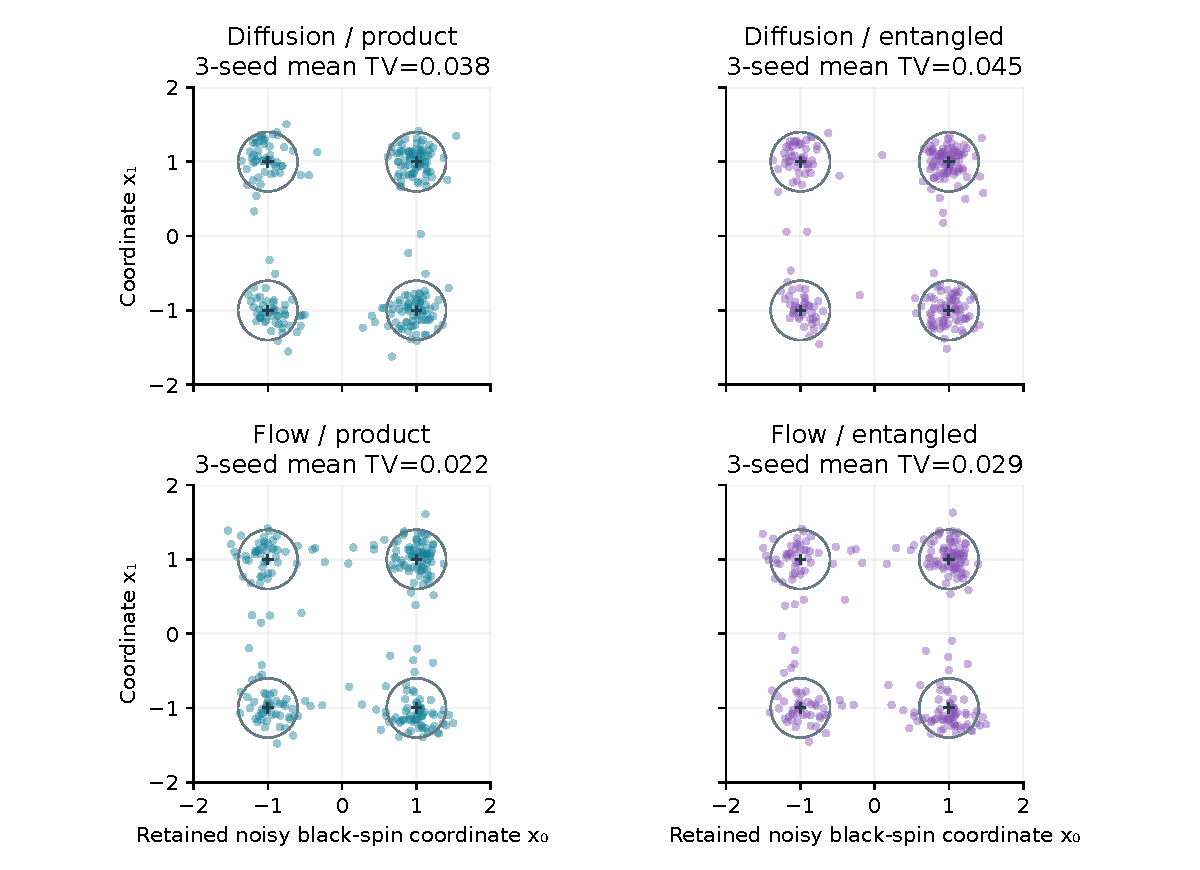
\includegraphics[width=.94\linewidth]{../book/figures/learned-generative.pdf}}
\caption{Actual final samples from seed20261104, with exact mixture centers and two-standard-deviation circles. Titles report mean sign-law TV over three seeds. The product control is competitive; no entanglement advantage is inferred.}
\end{figure}

\subsection{A coherent learned purification flow}
We separately implement quantum evolution, without identifying it with the
classical samplers. Exact depolarizing diffusion is
\[
 D_t(\rho_R)=e^{-t}\rho_R+(1-e^{-t})I_4/4.
\]
It preserves trace and positivity and satisfies $D_sD_t=D_{s+t}$ by direct
substitution. Its linear inverse on all matrices is not positive:
$D_t^{-1}(P)=e^tP-(e^t-1)I_4/4$ has a negative eigenvalue on the orthogonal
complement of any rank-one projection $P$ when $t>0$.
Thus a learned inverse cannot be a universal deterministic physical channel.

For a constructive state-preparation benchmark, take the family
$R_t=(1-t)I_4/4+t\rho_R$, $0\leq t\leq1$, and its canonical purification
$|\Psi_t\rangle=\operatorname{vec}\sqrt{R_t}$ in
$\mathbb C^4\otimes\mathbb C^4$. It is normalized because
$\|\sqrt{R_t}\|_F^2=\operatorname{tr}R_t=1$.
The initial purification is two Bell pairs. We train a six-block four-qubit
circuit: each block conjugates local $R_Y$ rotations by a fixed CNOT network
and its inverse; angles are $t\theta+t^2\omega$. All blocks are identity at
the control time zero. The 48 learned controls are trained against full
known purification states, using the fidelity loss. This ideal supervision
is stronger than access to measured samples and is accounted for explicitly.

An RTX4090 run of 2,000 steps, batch 64, gives minimum fidelity $0.999903$
on a 33-point grid and maximum reduced-density Frobenius error $0.009642$.
The reduced state is obtained by an actual ancilla partial trace and passes
trace/positivity checks. These are grid diagnostics, not a uniform or
out-of-family guarantee. The construction is a learned coherent control
path for known targets, not a universally learned inverse to depolarization.
Its full 76-gate replay and intermediate complex states are exported to the
same numerical architecture inspector as the other models.

\subsection{Width, fields, RG and arithmetic obligations}
Proposition~\ref{lf:kernel} fixes which width is being increased: the number
of independent one-qubit features, with only their readout trained.
At initialization let $a_r\sim N(0,1)$ be independent standard centered
readout coefficients, independent of the frozen features. Conditional
finite-dimensional outputs are then exactly centered Gaussian with
covariance $K_m$. The almost-sure kernel
convergence implies convergence of these finite-dimensional characteristic
functions to the Gaussian law with covariance $K$. This proves the specified
finite-dimensional GP limit. It does not prove tightness in a function-space
norm, parameter-feature learning, a many-qubit limit or a continuum QFT.
For frozen $K_m$, squared-loss gradient flow gives
$\dot r=-K_mr$, whose eigencomponents decay at their kernel eigenvalues.
A zero eigenvalue leaves a nonzero residual unchanged.

The executable width experiment fits the existing exact 32-configuration
\emph{classical} black-spin-decimated action on genus two, including its
constant. This is a second true RG teacher, distinct from the quantum
white-spin partial trace above. With 96 parameter triples for training,
32 for testing, eight feature seeds and ridge $10^{-5}$, widths 16 and
4,096 give mean relative kernel errors $0.2990$ and $0.01726$ and mean
full-action test MSE $0.02005$ and $0.000743$. The limiting RBF readout is
also evaluated. Finite numerical convergence supports the implementation;
the proposition supplies the limit proof. Quantum NTK literature requires
its own parameterization, ensemble and lazy/large-width hypotheses
\cite{LFQNTK,LFNTK}.

\begin{figure}[htbp]\centering
\IfFileExists{figures/learned-width-flow.pdf}{\includegraphics[width=.94\linewidth]{figures/learned-width-flow.pdf}}{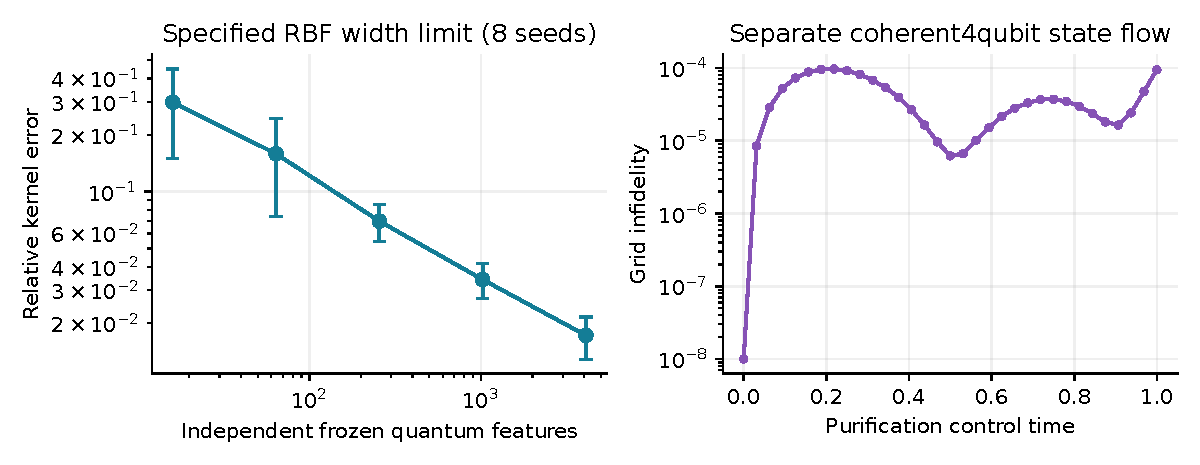
\includegraphics[width=.94\linewidth]{../book/figures/learned-width-flow.pdf}}
\caption{Left: eight-seed frozen-feature kernel errors, with sample standard deviations. Right: the separate learned coherent purification flow, evaluated on33time points. These are distinct width and quantum-control experiments.}
\end{figure}

For complex embeddings the Hermitian Gram form, realification
$A+iB\mapsto\left(\begin{smallmatrix}A&-B\\B&A\end{smallmatrix}\right)$,
and conjugation must be respected. An arbitrary real network on twice as
many channels need not be complex linear. In characteristic two,
$1+1=0$; an embedding into real vectors cannot be a unital field
homomorphism preserving that addition. Finite-field path algebras and
cellular/CSS computations are still meaningful, but Gaussian integration,
ordered Gibbs weights and real backpropagation do not transfer by renaming
the field. An explicit discrete learner over $\mathbb F_p$, $p=2,3,5$, uses
features $1,x,y,xy$ and coefficients searched in the finite field to learn
$f(x,y)=xy$. All $p^2$ inputs are verified; an affine-only learner has
nonzero minimum error. The trained map compiles to the permutation unitary
$U_f|x,y,z\rangle=|x,y,z+f(x,y)\bmod p\rangle$ on a complex Hilbert
space of dimension $p^3$. Retaining $x,y$ makes its inverse subtraction
explicit. This is reversible encoding of a field-valued polynomial learner,
not a field embedding into complex amplitudes or backpropagation in
$\mathbb F_p$. Its training is exact finite coefficient search.
A tropical semiring is not a field; coefficient cancellation,
valuation signs and the underlying valued algebra must be specified.

For GRH, each architecture offers an experimentally testable role:
quantum features can parameterize candidate metrics or probe observables;
graph tokens can encode actual local incidence, masks and monodromy;
tropical attention can search extremal valuations or active constraints;
flow/diffusion can propose continuous operator/control parameters;
RG can organize a genuine hierarchy of coarse actions. None of these
roles proves that its Gram matrix is the arithmetic positive metric.
One must still construct the arithmetic object with correct conductor,
gamma factors, zero divisor and domain, prove compact-uniform control and
zero location, and keep Dirichlet, Hecke, Dedekind and Artin hypotheses
separate. A learned candidate is accepted only after its exact defining
equations and analytic estimates are supplied.

\section{Covers, paths, pants and quantum games}\label{lf:geometry}
\subsection{Which free group and which universal cover?}
Write $F_2=\langle x,y\rangle$, $\mathbb F_2$ and $\widehat F_2$ for the
free group, coefficient field and profinite completion, respectively.
For a theta graph with vertices $A,B$ and edges $a,b,c$, an explicit cover
has vertices $(g,A),(g,B)$, $g\in F_2$, and edges
\[
 a:(g,A)-(g,B),\qquad b:(g,A)-(gx,B),\qquad c:(g,A)-(gy,B).
\]
Left multiplication is the deck action. Contracting all $a$-edges produces
the usual four-regular Cayley tree of $F_2$; before contraction the graph is
three-regular. Equivalently, vertices are reduced nonbacktracking edge paths
from $A$, with an immediately reversed edge cancelled. This gives a tree
and unique path lifting in every length. Its radius-$r$ patch has
$1+3\sum_{k=0}^{r-1}2^k$ vertices, hence 766 at radius eight.
With a planar ribbon structure the abstract graph is a spine of a
topological pair of pants. The actual $m=3$ dessin instead has the ribbon
structure of a once-punctured torus. Forgetting the cyclic orders identifies
the abstract graphs, not these thickenings. Graph distance is not
automatically hyperbolic geodesic length.

For the contracted clean $m$-edge dessin there are two vertices and $m$
parallel edges, so $\pi_1$ is $F_{m-1}$ and the analogous universal tree is
$m$-regular. The new examples include $m=5,9$, of genus two and four.
Reinserting clean white bivalent vertices subdivides its edges.
Attaching the face to recover the compact surface introduces a relation;
the closed genus-two surface has its surface group and a disk universal
cover, not one of these graph trees. Separately,
$\mathbb P^1\setminus\{0,1,\infty\}$ has fundamental group $F_2$.
The unbranched cover induced by a clean dessin removes all preimages of
those three values. For our degree-$2m$ map there are $m+3$ punctures;
its Euler characteristic is $-2m$, not that of the dessin's one-skeleton.
Thus the occurrences of $F_2$ in monodromy, graph covers and arithmetic
profinite theory must not be silently identified.

\begin{figure}[htbp]\centering
\IfFileExists{figures/learned-covers.pdf}{\includegraphics[width=.94\linewidth]{figures/learned-covers.pdf}}{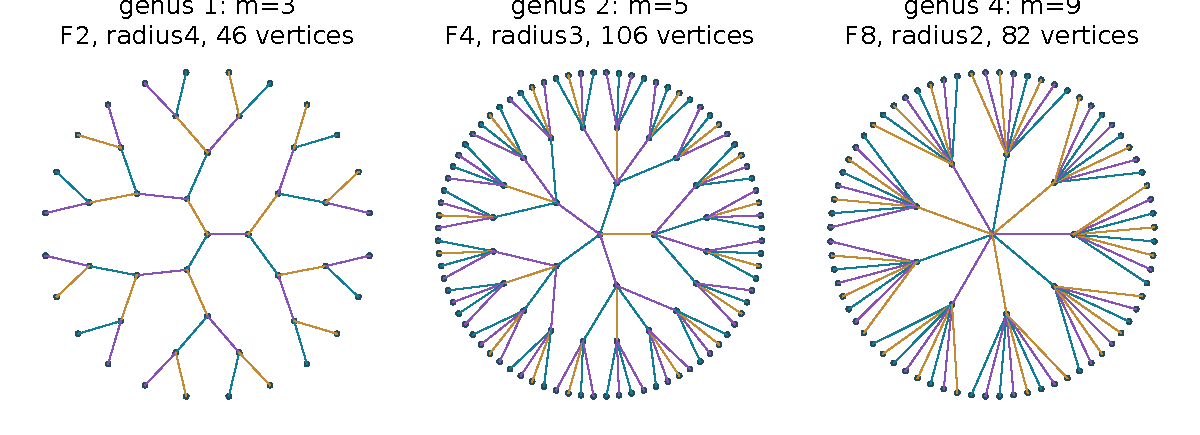
\includegraphics[width=.94\linewidth]{../book/figures/learned-covers.pdf}}
\caption{Finite windows of universal covers of contracted actual clean dessins. These are schematic graph trees, not uniformizing embeddings of the compact surfaces. Clean white bivalent vertices are suppressed.}
\end{figure}

For finite-supported representations of a suitably graded bound quiver,
pushdown maps split into deck-homogeneous blocks. The arrow equations
preserve the degree, and monomial zero relations are homogeneous. The
resulting Hom direct sum controls all deck pieces, not just degree one.
For an explicit graph-only diagnostic two lifted edge intervals have
upstairs endomorphism dimension two, but downstairs endomorphism dimension
four: the deck pieces have dimensions $2+1+1$. This graph-quiver calculation
is \emph{not} substituted for a dessin-algebra module example.
The actual infinite polynomial module examples below supply that part.
A Hom-controlled functor needs its specified exceptional/source/target
subcategory and control statement; exactness, a deck-sum formula or equal
dimensions alone is not an equivalence or an AR universality theorem.
A derived comparison must control all $\operatorname{Hom}(X,Y[n])$ and
composition, together with an actual derived/enhanced functor.

\subsection{Actual infinite-algebra path modules and unbounded resolutions}
To fix conventions, let $A_{\rm col}$ be the earlier rightmost-arrow-first
polynomial matrix algebra acting on left columns. Here we use travel-order
path multiplication and write $A_{\rm trav}=A_{\rm col}^{\rm op}$ for the
prose-identified bound-quiver algebra. Right $A_{\rm trav}$ representations
therefore encode the earlier covariant left-column representations.
There are vertices $i\in\mathbb Z/5$ and arrows $a_i,b_i:i\to i-1$, with
\[
 a_ib_{i-1}=b_ia_{i-1}=0.
\]
Both pure branch paths survive at every length. No arrow-truncated finite
algebra is being used. We work with ordinary polynomial modules, not with
all completed lattices or all infinite strings.

Put $P_i=e_iA_{\rm trav}$ and let $S_i$ be its residue simple.
The augmentation kernel is $a_iA\oplus b_iA$. Multiplication by an arrow
kills exactly the opposite-branch positive paths at its target, while each
surviving path has a distinct normal image. Its kernel is therefore the
right ideal generated by its unique forbidden successor, without cancellation.
Iteration yields a projective resolution with
\[
 P_0=P_i,\qquad P_n=P_{i-n}\oplus P_{i-n}\quad(n\geq1).
\]
The two arms are indexed by alternating-branch relation words. The
\emph{differential entry is the last arrow}, not the product of the zero
relation word. This kernel description proves exactness in every degree.
Applying Hom to a simple kills every arrow entry, hence
\[
 \dim\operatorname{Hom}(S_i,S_j)=\mathbf1_{i=j},\qquad
 \dim\operatorname{Ext}^n(S_i,S_j)=2\mathbf1_{j=i-n}\quad(n\geq1).
\]
Tensoring with the left residue simple gives the same Tor dimensions.
A graded version needs its internal degree shifts. In particular the
residue simples have infinite projective dimension in this ambient algebra.

Let $B$ be the one-arrow string supported at vertices zero and four, with
$a_0=1$ and every other arrow zero. Its presentation is
\[
 P_4\oplus P_3\xrightarrow{(b_0,\ a_0a_4)}P_0\longrightarrow B\longrightarrow0.
\]
The two images have disjoint normal-path support and span the kernel,
because $B$ retains exactly $e_0,a_0$. The next entries are $a_4$ on the
first arm and $b_3$ on the second; continue by their unique forbidden successors.
This gives an unbounded exact resolution by the same normal-path argument.
Full arrow-commuting equations give
\[
 \dim\operatorname{Hom}(B,B)=1,\quad
 \dim\operatorname{Hom}(S_0,B)=0,\quad
 \dim\operatorname{Hom}(B,S_0)=1,\quad
 \dim\operatorname{Hom}(S_4,B)=1.
\]
In the Hom complex for $\operatorname{Ext}^1(B,B)$ both adjacent
differentials vanish, so $\operatorname{Ext}^1(B,B)\simeq\mathbb Q$.
A concrete nonsplit self-extension has $\mathbb Q^2$ at zero and four,
$a_0=I_2$, $b_0=\left(\begin{smallmatrix}0&1\\0&0\end{smallmatrix}\right)$,
all other arrows zero. The first-coordinate submodule and quotient are $B$.
A section at vertex zero would lift the quotient basis to a vector with
second coordinate one; $b_0$ sends it to a nonzero first-coordinate vector,
contradicting commutation with the zero $b_0$ action on $B$. Thus $B$ is
not rigid in this actual ambient category. No almost-split universality
is inferred from this nonsplitting.

For finite-dimensional $N$ let $DN=\operatorname{Hom}_{\mathbb Q}(N,\mathbb Q)$.
On each finite idempotent projective the evaluation pairing identifies
$P\otimes_A DN$ with $D\operatorname{Hom}_A(P,N)$.
Dualization is exact on these finite-dimensional terms, so the resulting
complexes give
$\operatorname{Tor}^A_n(M,DN)\simeq D\operatorname{Ext}^n_A(M,N)$
for the stated finitely generated resolutions. In particular
$\operatorname{Tor}_1^A(B,DB)\simeq\mathbb Q$.
The exact program checks six source/target pairs through degree twelve,
all five simple-target formulas and 250 normal-kernel samples. The
unbounded resolution assertions rest on the normal-form proof, not on the
finite cutoff. These new homological proofs are prose/exact calculations;
full corresponding resolution objects are not yet Lean packaged.

A geometric path may label a string after specifying the ribbon structure,
relations and category. Turning it into a geodesic needs a metric and
appropriate boundary/stop data. Intersections compute morphisms only under
the hypotheses of an actual graded/Fukaya comparison. The homologically
smooth graded-gentle perfect-category theorems do not identify our entire
ordinary or completed module category with the Fukaya category by inspection
\cite{LFFukaya}. In particular the residue resolutions warn against
silently imposing smoothness or finite projective dimension.

\subsection{Pants tensors, physical dilation and sewing boundaries}
For $C=\mathbb Q[\epsilon]/\epsilon^2$, take
$\varepsilon(1)=0$, $\varepsilon(\epsilon)=1$. In the ordered bases
$(1,\epsilon)$ and $(1\otimes1,1\otimes\epsilon,
\epsilon\otimes1,\epsilon\otimes\epsilon)$, multiplication and
comultiplication are
\[
 \mu=\begin{pmatrix}1&0&0&0\\0&1&1&0\end{pmatrix},\qquad
 \Delta=\begin{pmatrix}0&0\\1&0\\1&0\\0&1\end{pmatrix}.
\]
The pairing is
$\left(\begin{smallmatrix}0&1\\1&0\end{smallmatrix}\right)$,
with determinant $-1$. Associativity follows from $\epsilon^2=0$;
coassociativity sends one to the three placements of a single one among
two $\epsilon$'s and sends $\epsilon$ to $\epsilon^{\otimes3}$.
On the four tensor basis vectors, all three maps in
\[
 \Delta\mu=(\mu\otimes I)(I\otimes\Delta)
          =(I\otimes\mu)(\Delta\otimes I)
\]
give, respectively, $1\otimes\epsilon+\epsilon\otimes1$,
$\epsilon\otimes\epsilon$, $\epsilon\otimes\epsilon$, and zero.
This proves the Frobenius identity. The unit and counit identities follow
directly on the same basis. These are exact oriented 2D TQFT gluing data
\cite{LFAbrams}, not a presumed positive Hilbert structure.

The handle map $H=\mu\Delta$ sends $1\mapsto2\epsilon$ and
$\epsilon\mapsto0$. Closed genus-$g$ contractions
$\varepsilon H^g\eta$ are $0,2,0,0,\ldots$.
The genus-two value really vanishes in this example. In characteristic
two the torus value also vanishes, illustrating a meaningful coefficient
change rather than an embedding-space relabelling.
After extending to $\mathbb C$ with the Euclidean metric,
$\Delta^*\Delta=\operatorname{diag}(2,1)$ and $\Delta\ne\mu^*$;
$\mu:\mathbb C^4\to\mathbb C^2$ is not an isometry.
The exact code constructs $K=\mu/\sqrt2$ and a $4\times4$ failure block
$L$ with $K^*K+L^*L=I_4$. Stacking them gives an isometry into
$\mathbb C^2\oplus\mathbb C^4$, extendable to a unitary with ancillas.
Its success probabilities on the four basis states are
$1/2,1/2,1/2,0$. Postselection implements $K$ with state-dependent success;
normalizing the selected outcome is not the original linear map $\mu$.

For a closed genus-$g\geq2$ surface a pants decomposition has $2g-2$
pieces and $3g-3$ sewn curves. Conformal sewing adds moduli-dependent
propagators and analytic consistency \cite{LFSegal}; string amplitudes
need worldsheet, ghost and integration data beyond this finite tensor.
A pants network or a hyperbolic graph is likewise not an AdS/CFT duality
or a Ryu--Takayanagi derivation \cite{LFRyu}. Such interpretations remain
specified research targets until their extra structure is constructed.
Arithmetic/anabelian reconstruction additionally requires arithmetic
profinite fundamental-group data and its Galois structure under the proper
field/curve hypotheses. Neither a discrete $F_2$ graph nor a coefficient
$\mathbb F_2$ module supplies that arithmetic extension \cite{LFAnabelian}.

\subsection{Quantum games and the Connes-embedding distinction}
For uniform input bits $x,y$, CHSH accepts outputs $u,v$ when
$u\oplus v=xy$. With $\pm1$ observables its success probability is
$1/2+\langle T\rangle/8$, where
\[
 T=A_0\otimes(B_0+B_1)+A_1\otimes(B_0-B_1).
\]
For a deterministic classical assignment one bracket vanishes and the
other is $\pm2$, giving success at most $3/4$; all sixteen assignments
are checked. On $|\Phi^+\rangle$, take $A_0=Z,A_1=X$,
$B_0=(Z+X)/\sqrt2,B_1=(Z-X)/\sqrt2$. Then
$T=\sqrt2(Z\otimes Z+X\otimes X)$ gives success
$(2+\sqrt2)/4$. For arbitrary self-adjoint involutions,
$T^2=4I-[A_0,A_1]\otimes[B_0,B_1]$ and each commutator has norm at most
two. Hence $\|T\|\leq2\sqrt2$, proving optimality.
The exact matrix checker verifies the entire spectrum
$\{-2\sqrt2,0,0,2\sqrt2\}$, not just a numerical sample.

MIP*$=$RE, in its pinned v4, gives an external unrestricted correlation
separation and a negative answer to Connes embedding \cite{LFMIP}.
We do not rerun its external formalization or claim a new proof of it.
CHSH has its optimum on two qubits and the same commuting optimum by
the preceding bound; it does not exhibit the general separation.
A learned game strategy is useful for finite witness search and checked
bounds, but unrestricted computability and dimension quantifiers cannot
be settled by a finite game simulation.

\subsection{Tropical accelerator reference designs and reproducibility}
The chip-design campaign pins twenty public repositories, twenty-four
focused document ranges and thirteen primary papers. It covers
AlphaChip/Circuit Training, independent macro-placement benchmarks,
OpenROAD-family flows, quantum layout and low-level control.
The source ledger records what was actually read, not a full audit or
reproduction of every model. An exact public identity for the phrase
``bare-metal Qiskit'' was not established; no repository was invented.

Three original executable references implement a masked signed max-plus
tile, an ordered mixed MAC/max-plus scheduler and a fail-closed synthetic
IQ steering controller. Wide addition precedes winner selection and final
saturation; earliest-index tie handling is explicit. Empty masks remain
invalid, not an extra candidate of value zero. The controller requires a
current calibration epoch, enough samples and a valid margin/deadline before
allowlisting a steering action. Checks include all 65,536 signed eight-bit
additions, 262,144 masked two-lane cases, reordered completions and twelve
negative controls. These are digital reference models, not synthesized
RTL, routed chips, measured RF feedback, power/area estimates or universal
hardware speedups. A tropical context block can avoid multiplications
inside that primitive while its projections, scores and other layers still
require their own arithmetic.

The Linux snapshot preserves the Mac project, source clones, histories,
checkpoints and environment archives. Linux GPU execution uses the existing
Torch CUDA environment and a separately approved isolated cuQuantum prefix;
macOS binaries are not treated as a Linux installation. The conda lock,
setup instructions, gate/head replay records and all failures are retained.
The on-page book contains one canonical laboratory for this chapter and
links all five new checkpoint architectures into the existing tensor
inspector. New physics, width and homological results have their explicit
prose/numerical/external status; selected earlier Lean components do not
constitute a full formalization of this extension or a proof of GRH.
